\section{实验验证}
\label{secExpValidation}

我们提出两个实验来证明拟议的控制器,同时也是为了强调上一节所讨论的确定的问题并不限于精心构建的数字模拟。
实验使用 Crazyflie 2.0 四轴飞行器进行,在室内运动捕捉空间中运行。
第一个实验演示了一个带着大的初始偏航误差的飞行器起飞。
在第二个实验中,模拟了大的干扰,以演示飞行器从大的初始误差中恢复。

飞行器采用简单的级联控制结构进行控制,其中期望的平动加速度由位置误差上的比例-微分控制器计算, 
\begin{align}
  \translAccDes := -\gainPos \mrb{\pos - \posDes} - \gainVel \dot{\pos}
\end{align}
根据期望的加速度,期望的方向被生成为最小旋转矩阵 $\rotMatDes$ ,对其来说 
\begin{align}
	\translAccDes = \frac{1}{\mass} \rotMatDes \thrustDir \thrustMagDes + \gravity
\end{align}
其中 $\thrustMagDes$ 是期望的推力量值,也是通过上述定义。 

注意,这是一个不复杂的控制结构,但它足以证明拟议的控制法。

\commentOut{
Specifically, in the experiments, the following constants are used:
\begin{align}
  & \gainPos = 2 \mathrm{s}^{-2}
  & \gainVel = 4\sqrt{2}\mathrm{s}^{-1}
\\&\gainAttRed = 167 \mathrm{s}^{-2} 
  &\gainAttYaw = 2 \mathrm{s}^{-1} 
\\&\gainAtt    = \diag{\gainAttRed,\gainAttRed,\gainAttYaw}
  &\gainRates  = \diag{33,33,2} \mathrm{s}^{-1}
\end{align}
}

\begin{figure}
  \centering
  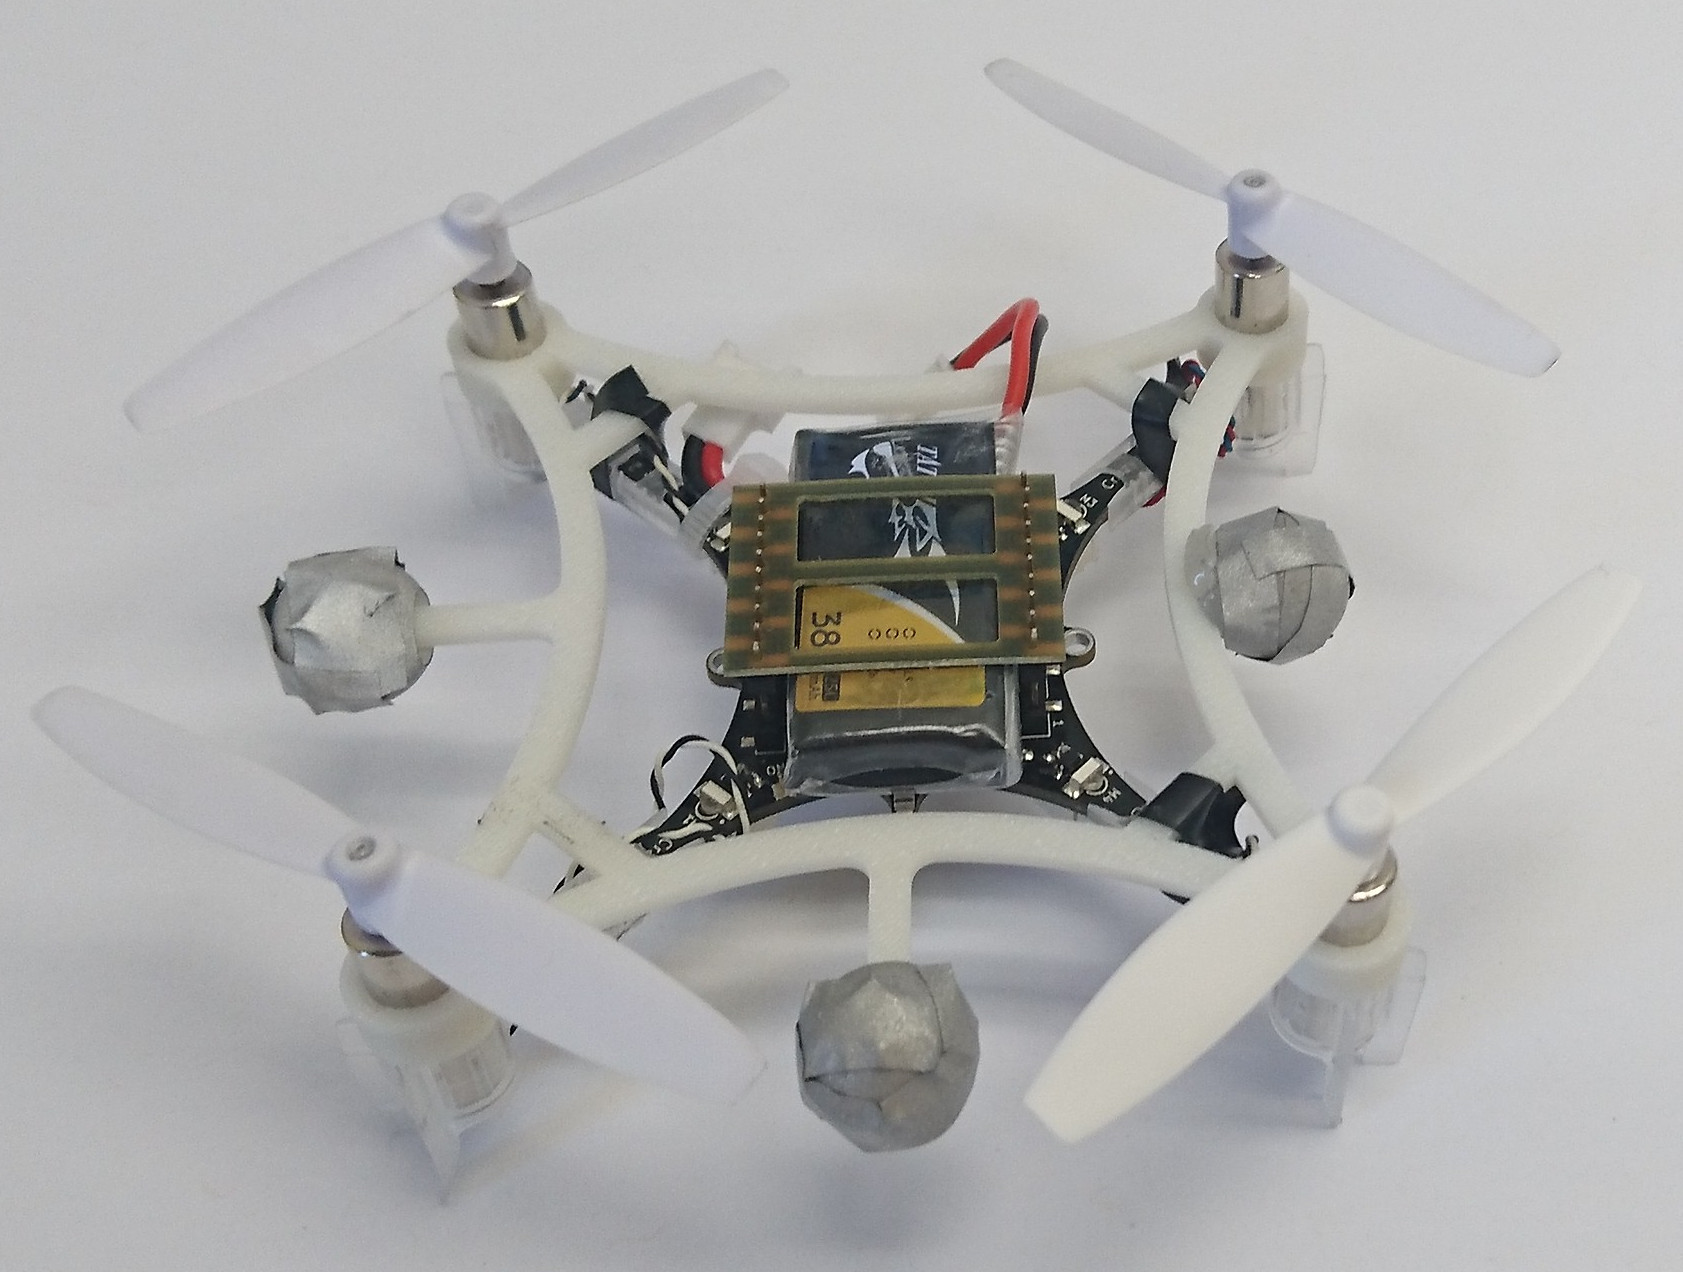
\includegraphics[width=0.7\linewidth]{Figures/quadcopter.jpg}
  \caption{
  实验中使用的四旋翼飞机,从螺旋桨尖到对置螺旋桨尖的尺寸约为 160mm。
  }
  \label{figExpQuad}
\end{figure}

\subsection{起飞时有大的偏航误差}
典型的多旋翼飞机的旋转对称性使得操作者很容易放置一个初始偏航误差较大的多旋翼飞机,这一点在 \figref{figExpQuad} 中可以看到。
为了说明这种误差的实际效果,一个四轴飞行器被命令起飞,并飞到一个高度为 1.5m 的设定点,在离起飞位置大约 0.5m 的水平距离。 
然而,四轴飞行器在初始化时有大的偏航误差(大约 177$^\circ$)。
在 \figref{figExpYaw} 中显示了新控制器和斜对称控制器的五个实验的位置轨迹。 
正如在 \secref{secPerfAdvantageTiltPrior} 中所预期的那样,斜对称控制器的表现非常差,在所有情况下,飞行器在到达目标点之前都会在目标点附近蜿蜒一段距离(如果它没有首先与墙壁相撞的话)。 
拟议的控制器没有表现出这种行为。

\begin{figure}
  \centering
  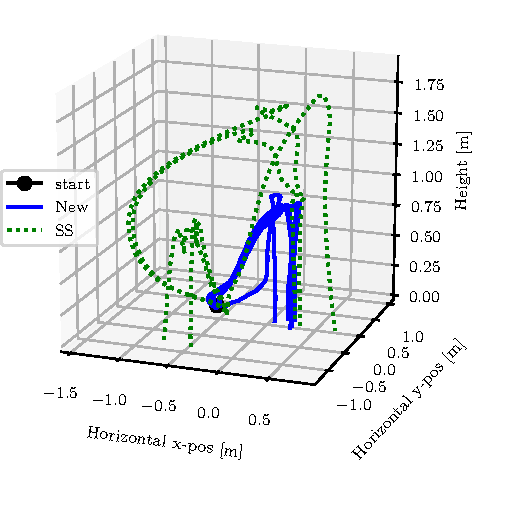
\includegraphics{Figures/Experiments/YawErrTakeoff/fig_traces.pdf}
  \caption{
  四轴飞行器从黑点开始,被命令沿 $x$ 方向水平飞行 0.5m,高度为 1.5m 的位置痕迹(对于多次实验)。
  四轴飞行器开始时有大的偏航误差。
  轨迹的变化是由于系统中的噪声造成的。
  }
  \label{figExpYaw}
\end{figure}

\subsection{从大的初始误差中恢复}
为了证明拟议的控制器在从大的干扰中恢复时的性能,我们进行了一系列的实验,在这些实验中,四旋翼飞机被用户抛到高空,而控制器只在飞行器超过一定的高度阈值时才启动。
这些实验的结果显示在 \figref{figExpLargeDisturbance} 中 -- 从图中可以看出,减小的姿态误差被迅速控制到零,而总的姿态误差可能衰减得更慢。 
这与之前的数值模拟示例的直觉相符。

\begin{figure}
  \centering
  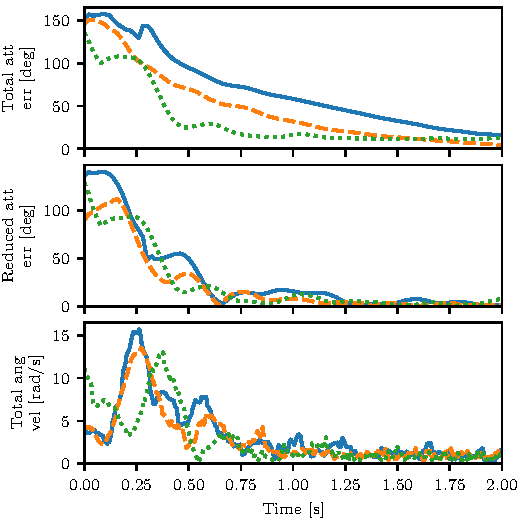
\includegraphics{Figures/Experiments/LargeDisturbances/fig_hists.pdf}
  \caption{
  一个飞行器在被用户扔到空中后,使用拟议的控制器从大的初始干扰中恢复的实验结果。 
  控制动作在时间 0 后立即开始,并且每种线条样式在三个图中标识相同的实验。
  姿态误差由运动捕捉数据估计,角速度由速率陀螺仪测量。
  }
  \label{figExpLargeDisturbance}
\end{figure}
